% Paquets généraux
\documentclass[a4paper,12pt,titlepage]{article}
\usepackage[T1]{fontenc}
\usepackage[utf8]{inputenc}
\usepackage[french]{babel}
\usepackage[gen]{eurosym}
%\usepackage[dvips]{graphicx}
\usepackage{fancyhdr}
\usepackage{pdfpages} 
\usepackage{multido}
\usepackage{hyperref}
%\usepackage{textcomp}
%\usepackage{aeguill}
\usepackage{schemabloc}
\usepackage[bitstream-charter]{mathdesign}
\usepackage{pstricks}
\usepackage{helvet}

\newcommand{\id}{30}
\newcommand{\nom}{Calculs d'hyperstatisme}
\newcommand{\sequence}{04}
\newcommand{\nomsequence}{Liaisons entre les solides}
\newcommand{\num}{03}
\newcommand{\type}{TD}
\newcommand{\descrip}{En appliquant les règles de la théorie des mécanisme, déterminer le degré d'hyperstatisme de plusieurs systèmes et proposer des solutions afin de diminuer ce degré}
\newcommand{\competences}{B2-12: Proposer une modélisation des liaisons avec leurs caractéristiques géométriques. \\ &  B2-13: Proposer un modèle cinématique paramétré à partir d'un système réel, d'une maquette numérique ou d'u \\ &  B2-17: Simplifier un modèle de mécanisme. \\ &  B2-18: Modifier un modèle pour le rendre isostatique.}
\newcommand{\nbcomp}{4}
\newcommand{\systemes}{E.P.A.S, Machine d'essai de traction}
\newcommand{\systemesnum}{14, 13}
\newcommand{\systemessansaccent}{E.P.A.S, Machine d'essai de traction}
\newcommand{\ilot}{3}
\newcommand{\ilotstr}{03}
\newcommand{\dossierilot}{\detokenize{Ilot_03 E.P.A.S, Machine d'essai de traction}}
\newcommand{\imageun}{EPAS}
\newcommand{\imagedeux}{Machine_dessai_de_traction}


\newcommand{\auteurun}{Renaud Costadoat}
\newcommand{\institute}{Lycée Dorian}


\usepackage{color}
\usepackage{xcolor}
\usepackage{colortbl}
\usepackage{helvet}
\renewcommand{\familydefault}{\sfdefault}
\usepackage{amsfonts}
\usepackage{amsmath}
%\usepackage{xspace}
\usepackage{varioref}
\usepackage{tabularx}
%\usepackage{floatflt}
\usepackage{graphics}
\usepackage{wrapfig}
\usepackage{textcomp}
\usepackage{tikz}
\usepackage{wrapfig}
\usepackage{gensymb}
\usepackage[european]{circuitikz}
\usetikzlibrary{babel}
\usepackage{ifthen}
\usepackage{cancel}
\usepackage{etoolbox}
\usepackage{multirow}
%\usepackage{boxedminipage}
\definecolor{gris25}{gray}{0.75}
\definecolor{bleu}{RGB}{18,33,98}
\definecolor{bleuf}{RGB}{42,94,171}
\definecolor{bleuc}{RGB}{231,239,247}
\definecolor{rougef}{RGB}{185,18,27}
\definecolor{rougec}{RGB}{255,188,204}%255,230,231
\definecolor{vertf}{RGB}{103,126,82}
\definecolor{vertc}{RGB}{220,255,191}
\definecolor{forestgreen}{rgb}{0.13,0.54,0.13}
\definecolor{blcr}{rgb}{0.59,0.69,0.84}
\definecolor{blfr}{rgb}{0.32,0.51,0.75}
\definecolor{orfr}{rgb}{0.90,0.42,0.15}
\definecolor{orcr}{rgb}{0.90,0.65,0.50}
\definecolor{orangef}{rgb}{0.659,0.269,0.072}
\definecolor{orange}{rgb}{0.58,0.35,0.063}
\definecolor{orangec}{rgb}{0.43,0.32,0.25}
\definecolor{rcorrect}{rgb}{0.6,0,0}
\definecolor{sequence}{rgb}{0.75,0.75,0.75}
\definecolor{competences}{rgb}{0.61,0.73,0.35}
\definecolor{grisf}{HTML}{222222}
\definecolor{grisc}{HTML}{636363}
\definecolor{normal}{HTML}{4087c4}
\definecolor{info}{HTML}{5bc0de}
\definecolor{success}{RGB}{92,184,92}
\definecolor{warning}{RGB}{240,173,78}
\definecolor{danger}{RGB}{217,83,79}
\hypersetup{                    % parametrage des hyperliens
    colorlinks=true,                % colorise les liens
    breaklinks=true,                % permet les retours à la ligne pour les liens trop longs
    urlcolor= blfr,                 % couleur des hyperliens
    linkcolor= orange,                % couleur des liens internes aux documents (index, figures, tableaux, equations,...)
    citecolor= forestgreen                % couleur des liens vers les references bibliographiques
    }

% Mise en page
\pagestyle{fancy}

\setlength{\hoffset}{-18pt}

\setlength{\oddsidemargin}{0pt} 	% Marge gauche sur pages impaire2s
\setlength{\evensidemargin}{0pt} 	% Marge gauche sur pages paires
\setlength{\marginparwidth}{00pt} 	% Largeur de note dans la marge
\setlength{\headwidth}{481pt} 	 	% Largeur de la zone de tête (17cm)
\setlength{\textwidth}{481pt} 	 	% Largeu\textbf{r de la zone de texte (17cm)
\setlength{\voffset}{-18pt} 		% Bon pour DOS
\setlength{\marginparsep}{7pt}	 	% Séparation de la marge
\setlength{\topmargin}{-30pt} 		% Pas de marge en haut
\setlength{\headheight}{55pt} 		% Haut de page
\setlength{\headsep}{20pt} 		% Entre le haut de page et le texte
\setlength{\footskip}{30pt} 		% Bas de\textbf{ page + séparation
\setlength{\textheight}{700pt} 		% Hauteur de l'icone zone de texte (25cm)
\setlength\fboxrule{1 pt}
\renewcommand{\baselinestretch}{1}
\setcounter{tocdepth}{1}
\newcommand{\cadre}[2]
{\fbox{
  \begin{minipage}{#1\linewidth}
   \begin{center}
    #2\\
   \end{center}
  \end{minipage}
 }
}


\newcommand{\titre}[1]
{\begin{center}
\cadre{0.8}{\huge #1} 
\end{center}
}

\newcounter{num_quest} \setcounter{num_quest}{0}
\newcounter{num_rep} \setcounter{num_rep}{0}

\newcommand{\question}[1]{\refstepcounter{num_quest}\par
~\ \\ \textbf{Question \arabic{num_quest} : }#1\label{q\the\value{num_quest}}\par
}

\newcommand{\reponse}[1]
{\noindent
\rule{\linewidth}{.5pt}\\
\textbf{Question \refstepcounter{num_rep}\ref{q\the\value{num_rep}} :} ~\ \\
#1}

% En tête et pied de page
\lhead{\nom}
\rhead{\includegraphics[width=2cm]{../../img/logo}}
\lfoot{Renaud Costadoat}
\cfoot{Page \thepage}

\fancypagestyle{correction}{%
  \fancyhf{}
  \lhead{\colorbox{danger}{\begin{minipage}{0.65\paperwidth} \textcolor{white}{\textbf{Correction}} \end{minipage}} }
  \rhead{\includegraphics[width=2cm]{../../img/logo}}
  \lfoot{Renaud Costadoat}
  \rfoot{\colorbox{danger}{\begin{minipage}{0.6\paperwidth} \begin{flushright}\textcolor{white}{\textbf{Correction}}\end{flushright} \end{minipage}} }}

\renewcommand{\footrulewidth}{0.4pt}

\usepackage{eso-pic}
\newcommand{\BackgroundPic}{%
\put(0,0){%
\parbox[b][\paperheight]{\paperwidth}{%
\vfill
\begin{center}
\hspace{0.5cm}\vspace{0.5cm}
\includegraphics[width=\paperwidth,height=\paperheight,%
keepaspectratio]{../../img/fond3}%
\end{center}
\vfill
}}}

\newcommand{\BackgroundPicdeux}{%
\put(25,-30){%
\parbox[b][\paperheight]{\paperwidth}{%
\vfill
\begin{center}
\includegraphics[width=\paperwidth,height=\paperheight,%
keepaspectratio]{../../img/fond4}%
\end{center}
\vfill
}}}

\begin{document}

\AddToShipoutPicture{\BackgroundPicdeux}

\pagestyle{fancy}

\section{Étude d'une tête de rotor d'hélicoptère}

\subsection{Présentation du produit}

\begin{figure}[htbp]
\begin{minipage}[c]{.40\linewidth}
\begin{center}
\includegraphics[width=\linewidth]{img/rotor.png}
\caption{Tête de rotor}
\label{fig:image1}
\end{center}
\end{minipage}
\hfill
\begin{minipage}[c]{.55\linewidth}
Le pilote d'un hélicoptère possède 3 systèmes principaux de commandes, le levier de pas général (ou collectif), le levier de pas cyclique (manche), et les palonniers (pédales). Le \og collectif \fg contrôle l'angle d'incidence commun de toutes les pales par l'intermédiaire des plateaux fixe et mobile, ce qui modifie la portance générée par le rotor. Le manche contrôle le pas cyclique qui introduit, par l'intermédiaire des mêmes plateaux, une action différenciée sur l'angle d'incidence de chaque pales.
\end{minipage}
\end{figure}

Les illustrations de la figure présentent le mécanisme du rotor principal d'un hélicoptère. On peut y distinguer les pièces principales suivantes :
\begin{itemize}
 \item Une pale (1), capable de pivoter autour d'un axe orthogonal à celui du rotor,
 \item Une biellette (2), chargée de transmettre le mouvement du plateau mobile (6) à la pale,
 \item Une biellette de commande (3), permettant de soulever ou d'incliner le plateau fixe (5),
 \item Le compas mobile (4) qui solidarise l'axe du rotor avec le plateau mobile (6),
 \item Le plateau dit fixe (5), pouvant monter et descendre, ainsi que pivoter autour d'axes uniquement orthogonaux à celui du rotor. Il transmet le mouvement des biellettes de commande au plateau mobile,
 \item Le plateau mobile (6) possède, en plus des mouvements du plateau fixe, la capacité de tourner sur lui-même, puisqu'il est entraîné par l'axe du rotor par l'intermédiaire du compas mobile. Il repose sur le plateau fixe (articulation avec roulements). Le plateau mobile est chargé de donner une inclinaison (variable ou non) aux pales, en agissant sur les biellettes.
\end{itemize}

\clearpage

\paragraph{Question 1:} Recopier au tableau et compléter le diagramme de contexte du système \og Tête de rotor \fg.

\begin{center}
\ifdef{\public}{\includegraphics[width=0.5\linewidth]{img/Helico_contexte_vide}}{\includegraphics[width=0.5\linewidth]{img/Helico_contexte}}
\end{center}

\paragraph{Question 2:} Recopier au tableau et compléter le diagramme des cas d'utilisation du système \og Tête de rotor \fg.

\begin{center}
\ifdef{\public}{\includegraphics[width=0.4\linewidth]{img/Helico_Cas_Utilisation_vide}}{\includegraphics[width=0.4\linewidth]{img/Helico_Cas_Utilisation}}
\end{center}

\paragraph{Question 3:} Compléter le diagramme des exigences d'utilisation du système \og Tête de rotor \fg. Trouver les composants liés par la relation \og satisfy \fg avec les exigences de ce diagramme.

\begin{center}
\ifdef{\public}{\includegraphics[width=0.5\linewidth]{img/Helico_exigences_vide}}{\includegraphics[width=0.5\linewidth]{img/Helico_exigences}}
\end{center}

\newpage

\section{Étude d'une fixation de ski}

\subsection{Présentation du produit}

\begin{figure}[htbp]
\begin{minipage}[c]{.40\linewidth}
\begin{center}
\includegraphics[width=\linewidth]{img/ski1.png}
\caption{Fixation de ski: perspective}
\label{fig:image2}
\end{center}
\end{minipage}
\hfill
\begin{minipage}[c]{.55\linewidth}
Les différentes classes d'équivalence du système:
\begin{enumerate}
 \item Le bâti (0) = {2, 7, 11, 12, 13},
 \item Talonnière (I) = {1, 15},
 \item Piston (II) = {3},
 \item La vis (III) = {6, 8},
 \item Ecrou (IV) = {4, 5}.
\end{enumerate}
\end{minipage}
\end{figure}

\begin{figure}[htbp]
\begin{minipage}[c]{.40\linewidth}
\begin{center}
\includegraphics[width=\linewidth]{img/ski2.png}
\caption{Fixation de ski: Vue de côté}
\label{fig:image3}
\end{center}
\end{minipage}
\hfill
\begin{minipage}[c]{.55\linewidth}
\begin{center}
\includegraphics[width=\linewidth]{img/ski3.png}
\caption{Fixation de ski: Graphe des liaisons}
\label{fig:image4}
\end{center}
\end{minipage}
\end{figure}

\paragraph{Question 1:} Recopier au tableau et compléter le diagramme de contexte du système \og Fixation de ski \fg.

\begin{center}
\ifdef{\public}{\includegraphics[width=0.5\linewidth]{img/Fixation_contexte_vide}}{\includegraphics[width=0.5\linewidth]{img/Fixation_contexte}}
\end{center}

\paragraph{Question 2:} Recopier au tableau et compléter le diagramme des cas d'utilisation du système \og Fixation de ski \fg.

\begin{center}
\ifdef{\public}{\includegraphics[width=0.4\linewidth]{img/Fixation_use_case_vide}}{\includegraphics[width=0.4\linewidth]{img/Fixation_use_case}}
\end{center}

\paragraph{Question 3:} Compléter le diagramme des exigences d'utilisation du système \og Fixation de ski \fg. Trouver les composants liés par la relation \og satisfy \fg avec les exigences de ce diagramme.

\begin{center}
\ifdef{\public}{\includegraphics[width=0.5\linewidth]{img/Fixation_exigences_vide}}{\includegraphics[width=0.5\linewidth]{img/Fixation_exigences}}
\end{center}

\newpage

\section{Étude d'une paire de lunettes 3D}

\subsection{Présentation du produit}

\begin{figure}[htbp]
\begin{minipage}[c]{.40\linewidth}
\begin{center}
\includegraphics[width=\linewidth]{img/tele.jpg}
\caption{Téléviseur 3D}
\label{fig:image5}
\end{center}
\end{minipage}
\hfill
\begin{minipage}[c]{.55\linewidth}
La télévision en relief, ou télévision en 3D, est un terme commercial pour les techniques de stéréoscopie mises en \oe uvre pour diffuser des images procurant des effets de profondeur et de jaillissement. Depuis les années 2000, les recherches sur la télévision stéréoscopique et la télévision haute définition sont menées conjointement.
\end{minipage}
\end{figure}

\begin{figure}[htbp]
\begin{minipage}[c]{.40\linewidth}
\begin{center}
\includegraphics[width=\linewidth]{img/cine.jpg}
\caption{Cinéma Imax 3D}
\label{fig:image6}
\end{center}
\end{minipage}
\hfill
\begin{minipage}[c]{.55\linewidth}
\begin{center}
\includegraphics[width=0.5\linewidth]{img/lunettes.jpg}
\caption{Lunettes 3D}
\label{fig:image7}
\end{center}
\end{minipage}
\end{figure}

\paragraph{Question 1:} Recopier au tableau et compléter le diagramme de contexte du système \og Lunettes 3D \fg.

\begin{center}
\ifdef{\public}{\includegraphics[width=0.5\linewidth]{img/Lunettes_contexte_vide}}{\includegraphics[width=0.5\linewidth]{img/Lunettes_contexte}}
\end{center}

\paragraph{Question 2:} Recopier au tableau et compléter le diagramme des cas d'utilisation du système \og Lunettes 3D \fg.

\begin{center}
\ifdef{\public}{\includegraphics[width=0.4\linewidth]{img/Lunettes_use_case_vide}}{\includegraphics[width=0.4\linewidth]{img/Lunettes_use_case}}
\end{center}

\paragraph{Question 3:} Compléter le diagramme des exigences d'utilisation du système \og Lunettes 3D \fg. Trouver les composants liés par la relation \og satisfy \fg avec les exigences de ce diagramme.

\begin{center}
\ifdef{\public}{\includegraphics[width=0.5\linewidth]{img/Lunettes_exigences_vide}}{\includegraphics[width=0.5\linewidth]{img/Lunettes_exigences}}
\end{center}

\newpage

\section{Étude d'un poste d'imprégnation}

\subsection{Présentation de l'entreprise}

La Société des Moteurs Électriques de Normandie (SMEN) fabrique des moteurs électriques utilisés principalement dans l'industrie du froid (réfrigérateurs, conditionnement d'air, chambres froides,...) mais aussi dans d'autres applications (ventilateurs, robots ménagers,...).

\subsection{Présentation du produit}

Le moteur fabriqué est un moteur asynchrone. Il est constitué d'un stator, dont les bobines créent le champ magnétique tournant et d'un rotor à cage d'écureuil.

\subsection{La fabrication du stator}

\begin{figure}[htbp]
\begin{minipage}[c]{.30\linewidth}
\begin{center}
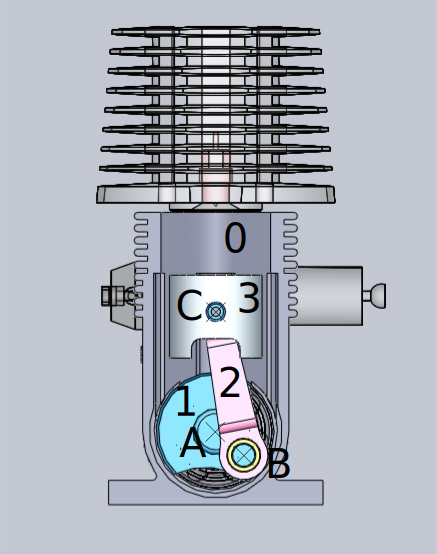
\includegraphics[width=\linewidth]{img/moteur.jpg}
\caption{Moteur électrique}
\label{fig:impre}
\end{center}
\end{minipage}
\hfill
\begin{minipage}[c]{.65\linewidth}
Le stator est constitué d'une armature métallique sur laquelle sont installés les bobinages. Le cycle de fabrication est le suivant:
\begin{itemize}
 \item bobinage de l'armature,
 \item préformage,
 \item lignature,
 \item formage,
 \item contrôle électrique,
 \item \textit{imprégnation},
 \item polymérisation,
 \item câblage,
 \item contrôle électrique.
\end{itemize}
\end{minipage}
\end{figure}


Nous allons étudier le poste d'imprégnation.

\subsection{Le poste d'imprégnation}

\begin{figure}[htbp]
\begin{minipage}[c]{.65\linewidth}
L'imprégnation consiste à tremper le stator dans un bac de vernis puis à éliminer l'excédent par centrifugation. Ce vernis est ensuite solidifié par échauffement à 180°C durant la phase de polymérisation.

Le but de l'imprégnation est de coller les fils électriques entre eux pour améliorer l'échange thermique et réduire l'échauffement du moteur. L'imprégnation améliore ainsi la fiabilité des moteurs.

L'installation est constituée de deux ensembles distincts:
\begin{itemize}
 \item Le manipulateur de chargement,
 \item L'unité d'imprégnation.
\end{itemize}
\end{minipage}
\hfill
\begin{minipage}[c]{.30\linewidth}
\begin{center}
\includegraphics[width=\linewidth]{img/impregnation.jpg}
\caption{Imprégnation d'un moteur}
\label{fig:impre0}
\end{center}
\end{minipage}
\end{figure}

L'alimentation et l'évacuation, en stators, du poste d'imprégnation s'effectuent sur 2 convoyeurs à chaînes \og en écailles \fg. Les pièces sont posées sur des palettes rectangulaires en plastique.

\subsubsection{Le manipulateur de chargement}
Le manipulateur permet le chargement et le déchargement d'un stator à la fois. Il est constitué d'un chariot à mouvement horizontal, d'une colonne à mouvement vertical, d'un poignet rotatif et d'une pince. Le serrage s'effectue sur l'extérieur du stator.

\subsubsection{L'unité d'imprégnation}
L'unité d'imprégnation comporte deux sous-ensembles, un sous-ensemble assurant le positionnement des stators et un sous-ensemble assurant l'imprégnation des stators.

\begin{itemize}
 \item Système de positionnement:
 
Il comporte une tête rotative à deux broches tournantes actionnée par un vérin pneumatique rotatif. Une broche est en position \og imprégnation \fg pendant que l'autre est en position \og chargement/déchargement \fg. Ce système permet d'opérer le trempage d'un stator fixé sur une broche pendant que l'on procède au déchargement d'un stator imprégné puis au chargement d'un stator non imprégné sur l'autre broche.
Les stators sont maintenus dans les broches au moyen de mandrins expansibles. Le serrage s'effectue par l'intérieur des stators.
 
 \item Système d'imprégnation:
  
L'imprégnation s'effectue en 2 temps. Le stator est d'abord trempé dans le fluide puis sorti du fluide et enfin \og égoutté \fg par centrifugation en faisant tourner les broches autour d'un axe vertical.
L'opération de trempage est réalisée par déplacement vertical du bloc de vernis.
Pendant la centrifugation, un carter escamotable permet la protection contre les projections. La rotation des broches est assurée par un moteur fixé sur le portique dont l'axe vient entraîner la broche en position imprégnation.
\end{itemize}

\paragraph{Question 1:} Recopier au tableau et compléter le diagramme de contexte du système \og poste d'imprégnation \fg.

\begin{center}
\ifdef{\public}{\includegraphics[width=0.5\linewidth]{img/Impregnation_contexte_vide}}{\includegraphics[width=0.5\linewidth]{img/Impregnation_contexte}}
\end{center}

\paragraph{Question 2:} Compléter le diagramme des exigences d'utilisation du système \og poste d'imprégnation \fg. Trouver les composants liés par la relation \og satisfy \fg avec les exigences de ce diagramme. 

\begin{center}
\ifdef{\public}{\includegraphics[width=0.9\linewidth]{img/Impregnation_exigences_vide}}{\includegraphics[width=0.9\linewidth]{img/Impregnation_exigences}}
\end{center}

\paragraph{Question 2:} Recopier au tableau et compléter le diagramme de bloc interne du système \og poste d'imprégnation \fg.

\begin{center}
\ifdef{\public}{\includegraphics[width=0.8\linewidth]{img/Impregnation_interne_vide}}{\includegraphics[width=0.8\linewidth]{img/Impregnation_interne}}
\end{center}

\newpage

~\

\newpage

\section{Étude d'une parabole}

\subsection{Présentation du produit}

\begin{figure}[htbp]
\begin{minipage}[c]{.65\linewidth}
Il s'agit d'un dispositif de réception satellite de chaînes numérique comme celles issues de \og bouquet \fg tels que Canal Satellite, etc...). 

Le problème est qu'à chaque satellite correspond un fournisseur. L'utilisation d'une parabole fixe, limite obligatoirement l'accès à un seul fournisseur. Ainsi, pour palier à cette contrainte, une parabole motorisée a été envisagée.
\end{minipage}
\hfill
\begin{minipage}[c]{.30\linewidth}
\begin{center}
\includegraphics[width=\linewidth]{img/parabole.jpg}
\caption{Parabole}
\label{fig:parabole1}
\end{center}
\end{minipage}
\end{figure}

\begin{figure}[htbp]
\begin{center}
\includegraphics[width=0.6\linewidth]{img/satellite.jpg}
\caption{Satellite émetteur}
\label{fig:parabole2}
\end{center}
\end{figure}

\paragraph{Question 1:} Recopier au tableau et compléter le diagramme des cas d'utilisation du système \og Parabole \fg.

\begin{center}
\ifdef{\public}{\includegraphics[width=0.4\linewidth]{img/Parabole_use_case_vide}}{\includegraphics[width=0.4\linewidth]{img/Parabole_use_case}}
\end{center}

\paragraph{Question 2:} Décrire les phases de vie du produit.

\newpage

\paragraph{Question 3:} Recopier au tableau et compléter le diagramme des exigences du système \og Parabole \fg à partir des Éléments du Milieu Environnant décrit dans la suite et sur le diagramme de contexte. Donner des valeurs numériques comme pour les exigences 1.1.2 et 1.1.3.

\begin{center}
\ifdef{\public}{\includegraphics[width=0.8\linewidth]{img/Parabole_exigences_vide}}{\includegraphics[width=0.8\linewidth]{img/Parabole_exigences}}
\end{center}

Les Éléments du Milieu Environnant sont:

\begin{enumerate}
 \item Support de fixation:
 \begin{itemize}
  \item Mur de matériaux solides (béton, brique, parpaing etc.) exceptés les matériaux fragiles (Placoplatre, brique de plâtre, etc.)
  \item Élément en bois plein (autre que compressé et contre plaqué),
  \item Éléments métalliques solidement fixés (rambarde),
  \item Cheminée, conduit d'aération solidement amarrée au reste de l'habitation.
 \end{itemize}
 \item Agent de maintenance
 \begin{itemize}
  \item Pas d'aptitude particulière nécessaire pour l'installation ou la désinstallation
 \end{itemize}
 \item Ambiants
 \begin{itemize}
  \item Rayonnement solaire (UV)
  \item Température de fonctionnement -20°C à 80°C
  \item Humidité et ruissellement d'eau	
  \item Vent régulier et rafales jusqu'à 120 km/h
 \end{itemize}
 \end{enumerate}
 
 \begin{minipage}{0.55\linewidth}
  \begin{enumerate}
  \setcounter{enumi}{3} 
 \item Énergie
 \begin{itemize}
  \item Source d'énergie classique, disponible dans une habitation, soit énergie électrique de nature EDF (220V, 50 Hz)
  \item Énergie mécanique éventuellement fournie par le matériel.
 \end{itemize}
 \item Satellites émetteurs
 \begin{itemize}
  \item Ensemble des satellites qui diffusent un bouquet numérique identifié par leurs coordonnées (latitude, longitude)
 \end{itemize}
 \item Téléspectateur
 \begin{itemize}
  \item Toute personne regardant la télé et en âge de faire fonctionner les appareils (7 ans)
 \end{itemize}
\end{enumerate}
 \end{minipage}
 \hfill
  \begin{minipage}{0.4\linewidth}
  \begin{center}
 \includegraphics[width=\linewidth]{img/Parabole_contexte}
\end{center}
 \end{minipage}

\newpage

\section{Colleuse de lamelles}

(Concours PCSI Mines AADN 2008)

\subsection{Introduction}

Le groupe TECH-INTER commercialise du matériel de laboratoire d'histopathologie. Cette spécialité médicale consiste à découper des tissus d'organes en fine épaisseur (4-5 mm). Ces tissus sont ensuite collés sur des lames de verres de 2 mm d'épaisseur, photo en haut à gauche de la figure \ref{fig:image101} puis colorés chimiquement dans un automate. Pour certains tissus, il est nécessaire de coller sur les tissus colorés une lamelle de verre de 0,3 mm d'épaisseur afin de les protéger, photo en haut à droite de la figure \ref{fig:image101}. Cette dernière opération est très délicate à effectuer manuellement et très longue, une étude pouvant comporter plusieurs centaines de lames.

\begin{figure}[htbp]
\begin{center}
\includegraphics[width=0.95\linewidth]{img/Image1.jpg}
\caption{Colleuse de lamelles}
\label{fig:image101}
\end{center}
\end{figure}

\begin{figure}[htbp]
\begin{minipage}[c]{.55\linewidth}
L'appareil appelé \og Colleuse de lamelle \fg automatise ce procédé, elle apparaît sur la figure \ref{fig:image102}.

\subsection{Préparation de l'appareil}

Les lames sont placées manuellement dans des paniers disposés dans des bacs inox remplis de toluène, figures \ref{fig:image102} et \ref{fig:image103}. Ces bacs sont positionnés sur un rail de transport puis glissés dans l'appareil (photos 4 et 5 document 2).

Un tiroir de rangement ayant été préalablement chargé en lamelles, un récipient de colle ayant été placé dans l'appareil et des racks de réception glissés dans l'élévateur, le cycle peut commencer.
\end{minipage}
\hfill
\begin{minipage}[c]{.40\linewidth}
\begin{center}
\includegraphics[width=0.8\linewidth]{img/colleuse.jpg}
\caption{Colleuse de lamelles}
\label{fig:image102}
\end{center}
\end{minipage}
\end{figure}

\newpage

\subsection{Cycle de collage}

L'opérateur programme la quantité de colle et le temps de séchage des lames collées puis appuie sur le bouton START. Le cycle se réalise alors automatiquement.

Le tapis roulant fait avancer le bac contenant le panier et un système de comptage détermine le nombre n de lames et leur position dans le panier. Un mécanisme bielle-manivelle muni d'une pince positionne une lame horizontalement et la dépose sur le support de lame.

Dans le même temps, une lamelle est aspirée du tiroir de rangement grâce à une pompe à vide puis est positionnée par un bras manipulateur au-dessus de la lame.

Un distributeur de colle dépose la colle sur la lame puis la lamelle descend sur la lame.

L'ensemble collé \og lame-lamelle \fg est stocké dans un rack par le support de lame.

\begin{figure}[htbp]
\begin{center}
\includegraphics[width=0.95\linewidth]{img/colleuse_exp.jpg}
\caption{Composants de la colleuse}
\label{fig:image103}
\end{center}
\end{figure}

\subsection{Partie opérative et partie commande}

Les actions de positionnement de la lame et de la lamelle sont réalisées grâce à des mécanismes de type :
\begin{itemize}
 \item \og bielle-manivelle \fg pour le positionnement de la lame,
 \item \og bras manipulateur \fg pour le positionnement de la lamelle figure \ref{fig:image102}.
\end{itemize}

Les actions permettant de compter les lames, de positionner les lames et les lamelles, de coller la lamelle sur la lame, de stocker les ensembles \og lame + lamelle collées \fg sont coordonnées et commandées par une unité centrale.

\begin{figure}[htbp]
\begin{center}
\includegraphics[width=0.5\linewidth]{img/colleuse_UC}
\caption{Diagramme des cas d'utilisation}
\label{fig:image104}
\end{center}
\end{figure}

\paragraph{Question 1:}
Reproduire et compléter au tableau le diagramme des cas d'utilisation de la figure \ref{fig:image104}.

\paragraph{Question 2:}
Reproduire et compléter au tableau le diagramme de bloc interne de la figure \ref{fig:image105}.

\paragraph{Question 3:}
Indiquer les éléments qui participent à la chaîne d'énergie du système. Pour chacun, indiquer dans quelle étape de la chaîne il intervient.

\paragraph{Question 4:}
Indiquer les éléments qui participent à la chaîne d'information du système. Pour chacun, indiquer dans quelle étape de la chaîne il intervient.

\begin{figure}[htbp]
\begin{center}
\includegraphics[width=0.95\linewidth]{img/colleuse_IBD}
\caption{Diagramme de bloc interne}
\label{fig:image105}
\end{center}
\end{figure}

\newpage

\section{Distributeur de boissons}

\begin{figure}[htbp]
\begin{minipage}[c]{.55\linewidth}
Un distributeur automatique est une machine qui permet d'obtenir des biens, sans intervention humaine (en libre-service), grâce aux techniques d'automatique.

Les machines les plus courantes sont le distributeur automatique de boissons chaudes, distribuant notamment le café mais on trouve aussi des distributeurs de boissons fraîches avec des ingrédients comme l'eau ou le thé.
\end{minipage}
\hfill
\begin{minipage}[c]{.40\linewidth}
\begin{center}
\includegraphics[width=0.9\linewidth]{img/Boissons.jpg}
\caption{Boissons dans un distributeur}
\label{fig:image106}
\end{center}
\end{minipage}
\end{figure}

\begin{figure}[htbp]
\begin{minipage}[c]{.40\linewidth}
\begin{center}
\includegraphics[width=0.9\linewidth]{img/piece.jpg}
\caption{Pupitre de commande}
\label{fig:image107}
\end{center}
\end{minipage}
\hfill
\begin{minipage}[c]{.55\linewidth}
Le fonctionnement est simple, l'utilisateur introduit un moyen de paiement (pièce, carte,...), passe une commande à l'aide d'une interface de communication, figure \ref{fig:image107}, puis sa commande lui est livré par le biai d'une ouverture dans le distributeur.
\end{minipage}
\end{figure}

\paragraph{Question 1:}

Proposer le diagramme des cas d'utilisation du système \og distributeur de boissons \fg.

\paragraph{Question 2:}

Proposer le diagramme de bloc interne du système \og distributeur de boissons \fg. Les sous-ensembles introduits seront les suivants:
\begin{itemize}
 \item \textit{Système de paiement},
 \item \textit{Carte de commande},
 \item \textit{Système de préparation de boisson}.
\end{itemize}

\paragraph{Question 3:}

Proposer le diagramme de bloc interne du système \og distributeur de boissons \fg. Les sous-ensembles introduits seront les suivants:
\begin{itemize}
 \item \textit{Système d'insertion de la monnaie},
 \item \textit{Contrôleur de monnaie},
 \item \textit{Stockage des pièces},
 \item \textit{Distributeur de monnaie}.
\end{itemize}

\newpage

\begin{figure}[htbp]
\begin{center}
\includegraphics[width=0.8\linewidth]{img/monnayeur.png}
\caption{Monnayeur d'un distributeur}
\label{fig:image108}
\end{center}
\end{figure}

\paragraph{Question 4:}
Indiquer les éléments qui participent à la chaîne d'énergie du système. Pour chacun, indiquer dans quelle étape de la chaîne il intervient.

\paragraph{Question 5:}
Indiquer les éléments qui participent à la chaîne d'information du système. Pour chacun, indiquer dans quelle étape de la chaîne il intervient.

\newpage

\section{Cellule de tri}

\subsection{Présentation}

Le traitement des ordures ménagères pose de nombreux problèmes dans les pays industrialisés.
Deux filières principales existent :
\begin{itemize}
 \item l'incinération,
 \item le recyclage.
\end{itemize}

Cette deuxième voie impose un tri sélectif de qualité. 

\begin{figure}[htbp]
\begin{minipage}[c]{.50\linewidth}
\begin{center}
\includegraphics[width=0.9\linewidth]{img/planeco.jpg}
\caption{Cellule de tri Planeco}
\label{fig:image109}
\end{center}
\end{minipage}
\hfill
\begin{minipage}[c]{.45\linewidth}
La filière de tri est basée sur une première séparation effectuée par les particuliers entre les ordures humides (végétaux, déchets de nourriture, etc.) et les ordures sèches (emballages, boites, bouteilles, etc.).
\end{minipage}
\end{figure}

\begin{figure}[htbp]
\begin{minipage}[c]{.4\linewidth}
Le dispositif étudié: PLANECO permet de trier automatiquement tous les emballages ménagers issus des collectes d'ordures sèches. La figure \ref{fig:image109} propose une vue générale d'une cellule de tri à quatre modules. La figure \ref{fig:image110} montre sur une première figure le détail d'un module de tri, sur une seconde figure le bras en cours de prise d'un objet creux.
\end{minipage}
\hfill
\begin{minipage}[c]{.55\linewidth}
\begin{center}
\includegraphics[width=0.9\linewidth]{img/planeco2.jpg}
\caption{Cellule de tri Planeco}
\label{fig:image110}
\end{center}
\end{minipage}
\end{figure}

\newpage

\subsection{Principe de fonctionnement}

La cellule de tri est alimentée au moyen d'une trémie de stockage équipée d'un tapis élévateur. 

Un dispositif magnétique «overband » élimine les objets ferreux puis un crible supprime les objets de trop petite taille. Un égreneur permet ensuite d'étaler les objets restant en vrac suivant une seule couche sur le tapis convoyeur d'un mètre de large. A l'entrée de chaque module on trouve donc sur un tapis une monocouche d'objets creux à trier.

Chaque module de tri assure sa fonction selon la procédure suivante :
\begin{itemize}
 \item une caméra vidéo couleur détermine d'abord la position, puis la forme et la couleur de l'objet visé,
 \item l'objet est ensuite saisi par le bras articulé au moyen d'une ventouse,
 \item lors de la saisie, un capteur électromagnétique situé dans la ventouse identifie les objets métalliques (principalement ceux en aluminium),
 \item si l'objet contient du métal, l'analyse d'images détermine son appartenance à un groupe connu: brique alimentaire, bouteille (conteneur de boissons) ou barquette,
 \item un capteur de verre, également situé dans la ventouse, reconnaît les verres par contact,
 \item tous les objets reconnus à ce stade sont déposés dans des goulottes appropriées,
 \item les emballages restant: en plastique ou en carton sont maintenus sur la ventouse,
 \item ils sont amenés par le bras à un spectromètre infrarouge, qui détermine le type de matière plastique de l'objet : PIC, PET, PERD tous recyclés ou autres plastiques non recyclés,
 \item un classificateur combine alors les données de vision et celles fournies par le spectromètre pour reconnaître par exemple un emballage en \og Polyéthylène (PET) azuré \fg,
 \item après identification, tous les objets pris sont déposés dans des goulottes différentes.
\end{itemize}

Le nombre de modules à installer dépend des quantités à traiter, on peut citer par exemple qu'une cellule à quatre modules permet de traiter 2000 tonnes de déchets hors verre par an pour un fonctionnement en deux fois huit heures par jour ce qui correspond à la « production » de déchets d'une population française de 130 000 habitants en fin des années 1990.

\paragraph{Question 1 :}

Construire le diagramme des cas d'utilisation du système.

\paragraph{Question 2:}

Proposer le diagramme de bloc interne du système \og cellule de tri \fg. Les sous-ensembles introduits seront les suivants:
\begin{itemize}
 \item \textit{Distributeur d'objets},
 \item \textit{Détecteur d'objets ferreux},
 \item \textit{Détecteur de petits objets},
 \item \textit{Système d'étalage des objets},
 \item \textit{Trieur d'objets}.
 \end{itemize}

\paragraph{Question 3:}
Indiquer les éléments qui participent à la chaîne d'énergie du système. Pour chacun, indiquer dans quelle étape de la chaîne il intervient.

\paragraph{Question 4:}
Indiquer les éléments qui participent à la chaîne d'information du système. Pour chacun, indiquer dans quelle étape de la chaîne il intervient.



\end{document}
